\documentclass[11pt]{article}
\usepackage[margin=1in]{geometry}
\usepackage{amsmath,amssymb,amsthm,graphicx,booktabs}
\usepackage[hidelinks]{hyperref}
\newtheorem{theorem}{Theorem}
\newtheorem{lemma}{Lemma}
\newcommand{\R}{\mathbb R}
\newcommand{\Z}{\mathbb Z}
\newcommand{\G}{\mathcal G}
\newcommand{\Mp}{M^p(\R)}
\newcommand{\Mr}{M^r(\R)}
\newcommand{\ip}[2]{\langle #1,#2\rangle}
\newcommand{\wh}{\widehat}
\setlength{\parindent}{0pt}
\setlength{\parskip}{0.62em}

\title{Conditional Critical Gabor Bases Give $M^p$ Counterexamples for Every $1<p<2$}
\author{Run \texttt{fa\_banach\_001}, lane 18}
\date{11 August 2026}

\begin{document}
\maketitle

\textbf{Status.} Candidate full negative answer to Question~5.1 of
arXiv:2408.16593, likely valid, for human review.

\section{Source question}

Yu asks whether, for $g,\gamma\in M^p(\R)$ with $1<p\leq2$, every critical
Gabor Schauder frame reconstruction that converges in $L^2$ (with respect to
some ordering) must converge unconditionally on $M^q$ for
$p\leq q\leq p'$.  The paper records the known $p=2$ obstruction of
Heil--Powell and explicitly leaves the existence of a counterexample for
every $1<p<2$ open \cite[Question~5.1]{Yu}.

\begin{center}
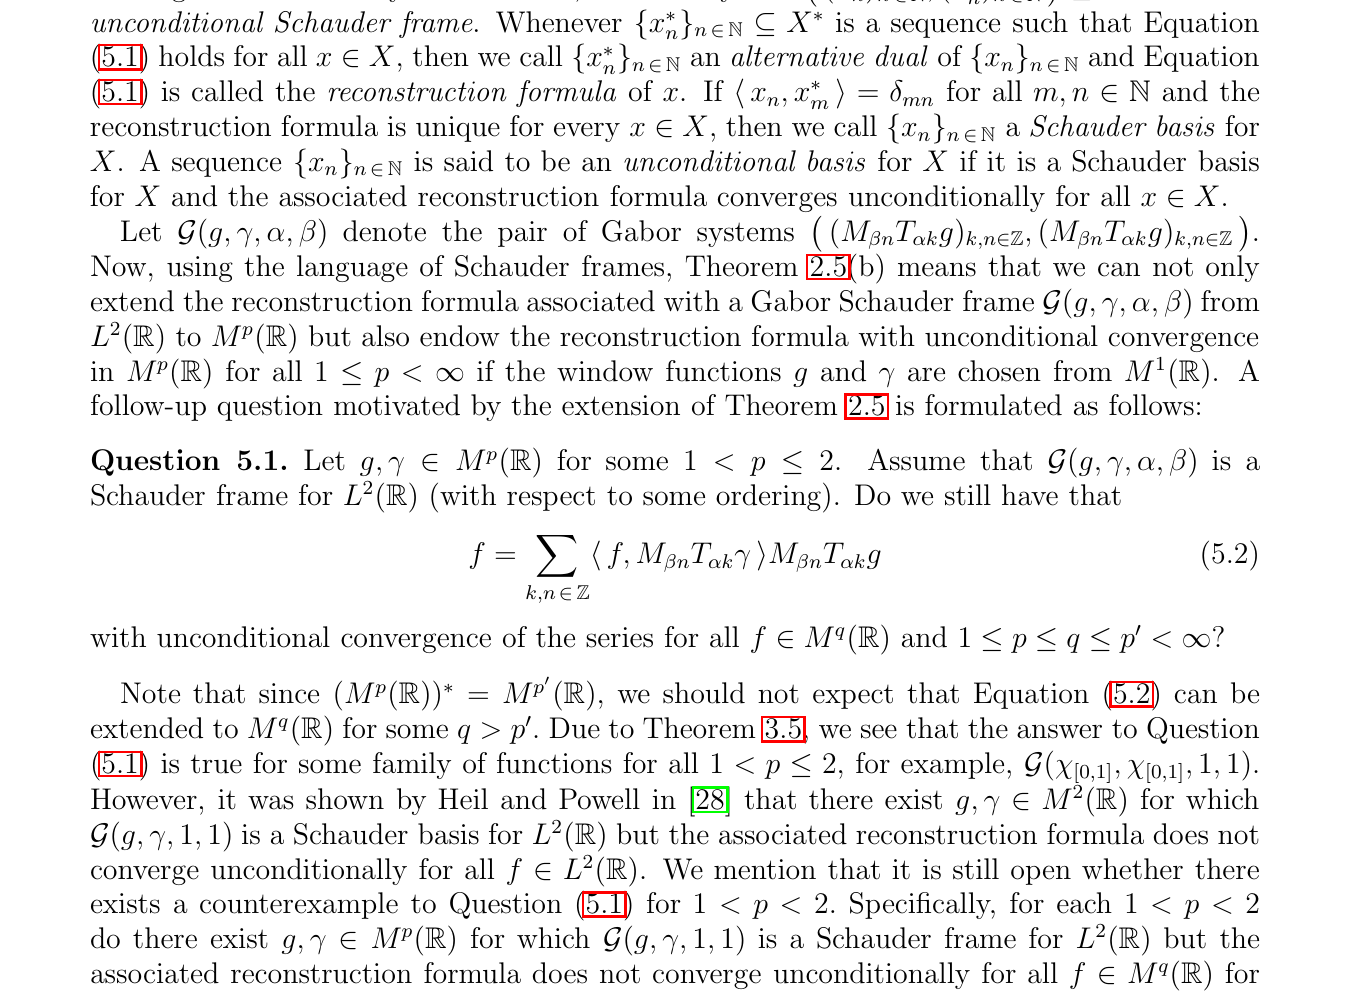
\includegraphics[width=0.75\textwidth]{figures/source_question_5_1.png}
\end{center}

Here $M^s=M^{s,s}$, $T_kf(t)=f(t-k)$, and
$M_nf(t)=e^{2\pi int}f(t)$.  We answer the question negatively already at
$q=2$.

\section{Claimed contribution}

\begin{theorem}\label{thm:main}
For every $1<p<2$ there are real, nonnegative, compactly supported windows
$g,\gamma\in M^p(\R)$ with the following properties.
\begin{enumerate}
\item For each Heil--Powell admissible rectangular enumeration
$\sigma\in\Lambda$, the pair
\[
 \bigl((M_nT_kg)_{(k,n)\in\Z^2},
       (M_nT_k\gamma)_{(k,n)\in\Z^2}\bigr),
\]
ordered by $\sigma$, is a Schauder basis together with its biorthogonal
dual, and hence a Schauder frame for $L^2(\R)$.
\item Its reconstruction does not converge unconditionally for every
$f\in L^2(\R)=M^2(\R)$.
\end{enumerate}
Consequently Question~5.1 of \cite{Yu} has a negative answer for every
$1<p<2$ (take $q=2\in[p,p']$).
\end{theorem}

The construction has a little more quantitative content.  If its endpoint
parameter is $0<\delta<1/2$, then, for $1<r\leq2$,
\begin{equation}\label{eq:threshold}
 \gamma\in M^r(\R)
 \quad\Longleftrightarrow\quad r(1-\delta)>1.
\end{equation}

\section{Proof intuition}

At critical density a window supported on one unit interval has Zak
transform equal to the window itself.  Heil and Powell observed that a
window which vanishes like $t^\delta$ at both endpoints has squared Zak
transform in the Muckenhoupt class $A_2$.  It therefore generates a Schauder
basis for their rectangular orderings, although it cannot be a Riesz basis
because its Zak transform approaches zero.

The unique dual window is the reciprocal $1/g$ on the unit interval.  Thus
the only missing issue in the 2024 question is whether that reciprocal has
the requested modulation-space regularity.  Its two endpoint singularities
are $t^{-\delta}$ and $(1-t)^{-\delta}$.  Their integer Fourier coefficients
have the same positive leading contribution, rather than cancelling:
\[
 \widehat\gamma(n)
 \sim 2\Gamma(1-\delta)(2\pi |n|)^{\delta-1}
       \sin\!\left(\frac{\pi\delta}{2}\right).
\]
The compact-support Fourier-coefficient characterization of $M^r$ then gives
the exact threshold \eqref{eq:threshold}.  Choosing
$\delta<1-1/p$ puts both basis windows in $M^p$, while conditionality of the
basis supplies the required failure at $q=2$.

\section{Construction and proof}

Fix $1<p<2$ and choose
\begin{equation}\label{eq:deltachoice}
 0<\delta<1-\frac1p.
\end{equation}
In particular $\delta<1/2$.  Choose a real, nonnegative function $g=g_\delta$
supported on $[0,1]$ such that
\begin{align*}
 g(t)&=t^\delta &&(0\leq t\leq1/4),\\
 g(t)&=(1-t)^\delta &&(3/4\leq t\leq1),
\end{align*}
$g(1-t)=g(t)$, $g$ is smooth on every compact subinterval of $(0,1)$,
and $g$ is bounded below by a positive constant on $[1/4,3/4]$.
Such a function is obtained by a symmetric smooth interpolation.  Define
\begin{equation}\label{eq:dual}
 \gamma(t)=
 \begin{cases}
  1/g(t),&0<t<1,\\
  0,&t\notin(0,1).
 \end{cases}
\end{equation}

\subsection*{The Schauder basis and its dual}

This is precisely the family in Heil--Powell's Example~5.11.  Their
Theorem~5.10 and the calculation $|Zg|^2=|g|^2\in A_2(\mathbb T^2)$ show that
$\G(g,1,1)$ is a Schauder basis of $L^2(\R)$ for every enumeration
$\sigma\in\Lambda$ \cite[Theorem~5.10 and Example~5.11]{HeilPowell}.

\begin{center}
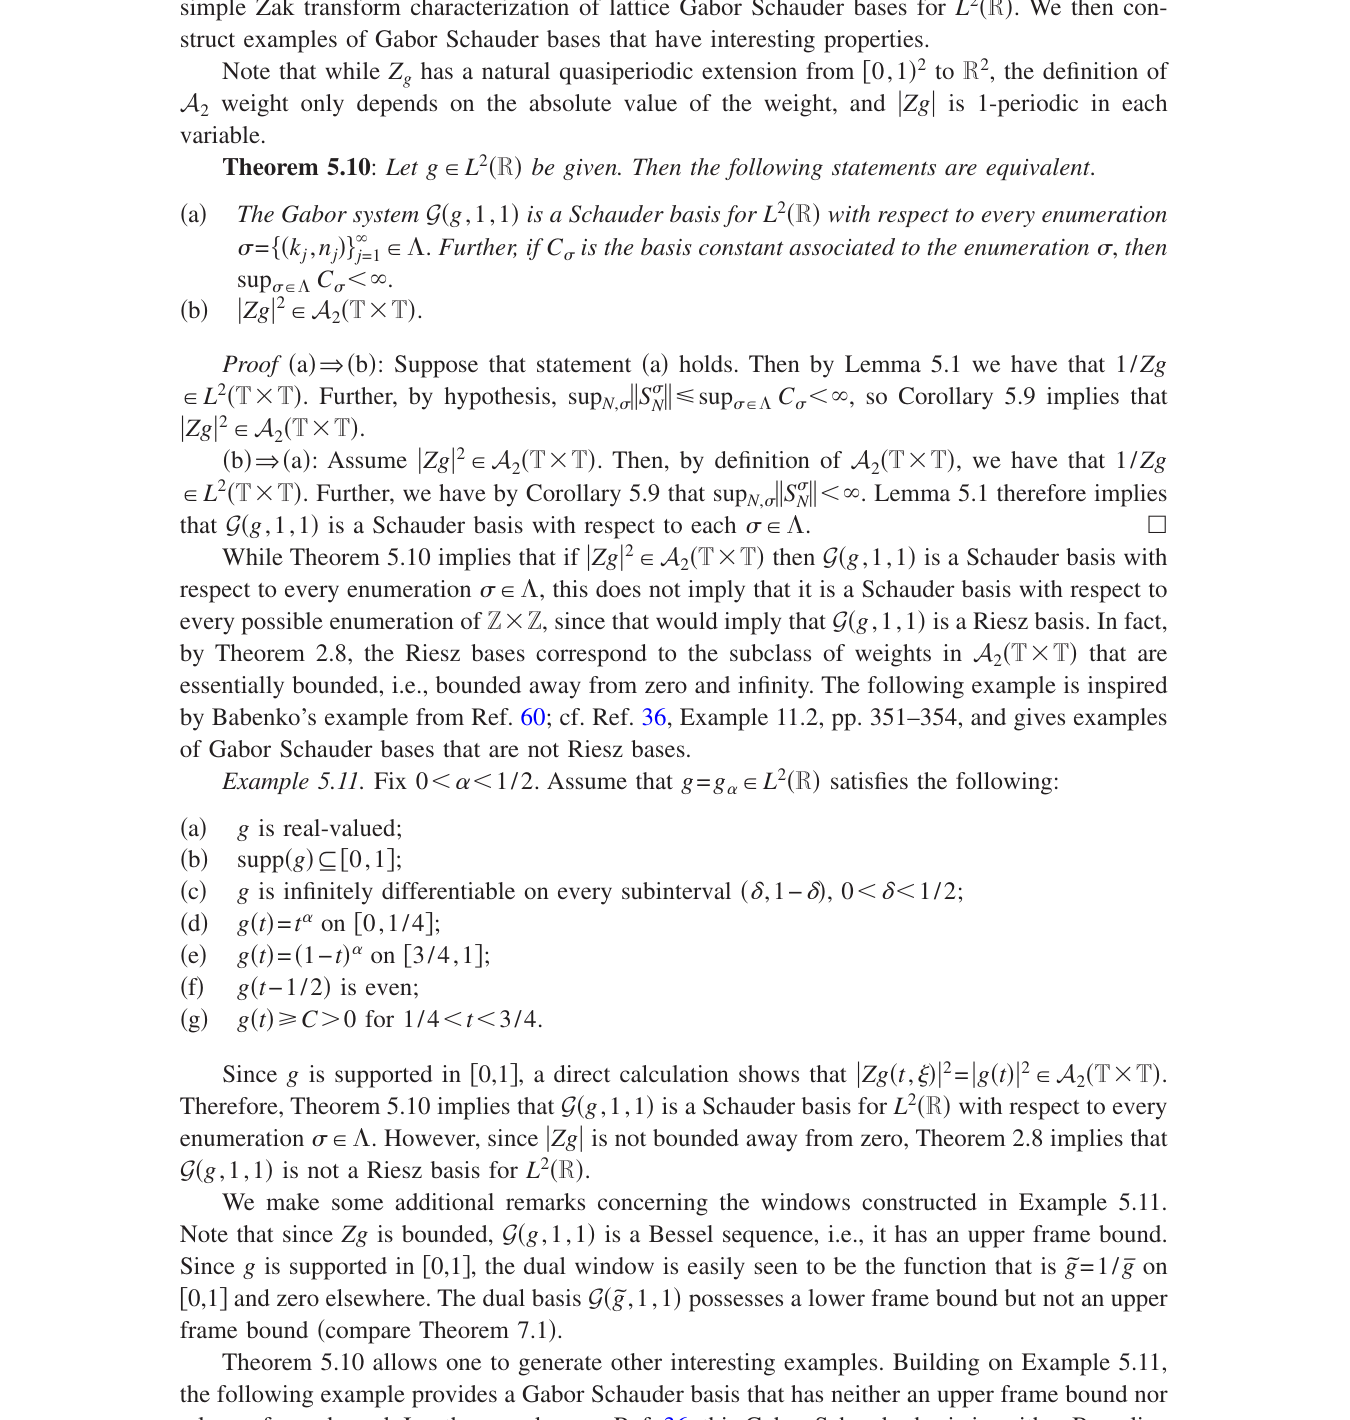
\includegraphics[width=0.72\textwidth]{figures/heil_powell_example_5_11.png}
\end{center}

Since $2\delta<1$, both $g$ and $\gamma$ lie in $L^2$.  The asserted
biorthogonality can also be checked directly.  If $k\neq\ell$, the interiors
of the supports of $T_kg$ and $T_\ell\gamma$ are disjoint.  If $k=\ell$,
then $g(t-k)\gamma(t-k)=1$ almost everywhere on $(k,k+1)$ and hence
\[
 \ip{M_nT_kg}{M_mT_k\gamma}
 =\int_k^{k+1}e^{2\pi i(n-m)t}\,dt=\delta_{nm}.
\]
Thus \eqref{eq:dual} is the unique biorthogonal window, exactly as noted by
Heil--Powell.

They also prove $g\in M^1(\R)$ \cite[Theorem~6.1]{HeilPowell}; in particular
$g\in M^p(\R)$.

\subsection*{The reciprocal belongs to $M^p$}

We record the endpoint calculation separately.

\begin{lemma}\label{lem:fourier}
For $\gamma$ in \eqref{eq:dual}, as $n\to+\infty$,
\begin{equation}\label{eq:asymptotic}
 \widehat\gamma(n)
 =C_\delta n^{\delta-1}+O(n^{-1}),
 \qquad
 C_\delta=
 2\Gamma(1-\delta)(2\pi)^{\delta-1}
 \sin\!\left(\frac{\pi\delta}{2}\right)>0.
\end{equation}
The coefficients at negative integers are their complex conjugates.
Consequently $(\widehat\gamma(n))_{n\in\Z}\in\ell^r$ if and only if
$r(1-\delta)>1$.
\end{lemma}

\begin{proof}
Take smooth endpoint cutoffs $\chi_0,\chi_1$ with $\chi_0=1$ near $0$,
$\chi_1(t)=\chi_0(1-t)$ near $1$, and disjoint supports.  By the exact
endpoint form of $g$,
\[
 \gamma(t)=\chi_0(t)t^{-\delta}
       +\chi_1(t)(1-t)^{-\delta}+h(t),
 \qquad h\in C_c^\infty(0,1).
\]
The standard endpoint oscillatory-integral formula (obtainable by the
scaling $u=2\pi nt$ followed by one integration by parts away from $0$)
gives
\begin{align*}
 \int_0^1\chi_0(t)t^{-\delta}e^{-2\pi int}\,dt
 &=\Gamma(1-\delta)(2\pi n)^{\delta-1}
   e^{-i\pi(1-\delta)/2}+O(n^{-1}),\\
 \int_0^1\chi_1(t)(1-t)^{-\delta}e^{-2\pi int}\,dt
 &=\Gamma(1-\delta)(2\pi n)^{\delta-1}
   e^{ i\pi(1-\delta)/2}+O(n^{-1}).
\end{align*}
In the second line the integer identity $e^{-2\pi in}=1$ has been used.
The Fourier transform of $h$ is rapidly decreasing.  Adding the two leading
terms and using
$\cos(\pi(1-\delta)/2)=\sin(\pi\delta/2)$ proves
\eqref{eq:asymptotic}.  Because $C_\delta>0$ and
$n^{-1}=o(n^{\delta-1})$, the claimed $\ell^r$ criterion follows by the
$p$-series test.
\end{proof}

Corollary~4.1 of \cite{Yu}, applied with $\alpha=\beta=1$, states that for
$1<r\leq2$ the $M^r$ norm is equivalent to the $\ell^r$ norm of the sampled
Fourier coefficients of the restrictions to the unit cells.  For clarity,
the converse membership implication can be read without presupposing that
$\gamma\in M^r$: take the ordinary Fourier partial sums
\[
 \gamma_N(t)=\mathbf 1_{[0,1]}(t)
       \sum_{|n|\leq N}\widehat\gamma(n)e^{2\pi int}.
\]
Each $\gamma_N$ lies in $M^r$, and Corollary~4.1 makes $(\gamma_N)$ Cauchy in
$M^r$ exactly when $(\widehat\gamma(n))\in\ell^r$.  Its $M^r$ limit agrees
with its $L^2$ limit $\gamma$ because $M^r\hookrightarrow M^2=L^2$ for
$r\leq2$.  The reverse implication follows by applying the same norm
equivalence directly.  Lemma~\ref{lem:fourier} therefore proves
\eqref{eq:threshold}.  The choice \eqref{eq:deltachoice} gives
$p(1-\delta)>1$, and hence $\gamma\in M^p(\R)$.

\subsection*{Failure of unconditional convergence}

Heil--Powell also show that this Schauder basis is not a Riesz basis: its Zak
transform is not bounded away from zero.  In a Hilbert space, an
unconditional Schauder basis is exactly a Riesz basis.  Therefore, for any
fixed admissible enumeration $\sigma\in\Lambda$, there is an $f\in L^2(\R)$
whose expansion in this basis is not unconditionally convergent.  Since
\[
 L^2(\R)=M^2(\R),\qquad p<2<p',
\]
the exponent $q=2$ is among those demanded in Question~5.1.  This completes
the proof of Theorem~\ref{thm:main}.

\section{Verification and scope}

The independent checks are recorded in \texttt{verification.md}.  The
accompanying script numerically checks the sign and scale of the endpoint
constant, but computation is not used in the proof.

This result answers the Schauder-frame Question~5.1.  It does \emph{not}
answer the separate question of whether the canonical dual of a genuine
redundant Gabor frame inherits a given modulation-space regularity: the
system here is a conditional Schauder basis and is not a Hilbert frame.

\section{Provenance and novelty check}

The conditional basis, its reciprocal dual, the $A_2$ argument, its failure
to be Riesz, and $g\in M^1$ are all due to Heil and Powell (2006).  The added
observation is the sharp Fourier-coefficient audit of $1/g$, which puts the
\emph{dual} in $M^p$ and thereby turns their construction into a
counterexample to the explicit 2024 question for every $1<p<2$.

A bounded search on 11 August 2026 covered the run's registry, solution,
attempt, and proof-gap indexes; exact-title and arXiv searches for
arXiv:2408.16593; searches combining ``Question 5.1'', ``Gabor Schauder
basis'', ``modulation space'', and ``Heil Powell''; and later related Gabor
unconditional-basis work.  The 2024 source has only its original arXiv
version, and no later paper found in that search states this answer.  This
supports, but cannot certify, novelty.

\begin{thebibliography}{9}
\bibitem{Yu}
P.-T. Yu,
\emph{Gabor frames with atoms in $M^q(\mathbb R)$ but not in
$M^p(\mathbb R)$ for any $1\leq p<q\leq2$},
arXiv:2408.16593 (2024),
\url{https://arxiv.org/abs/2408.16593}.

\bibitem{HeilPowell}
C. Heil and A. M. Powell,
\emph{Gabor Schauder bases and the Balian--Low theorem},
J. Math. Phys. \textbf{47} (2006), 113506.
\end{thebibliography}

\end{document}
